%%%%%%%%%%%%%%%%%%%%%%%%%%%%%%%%%%%%%%%%%
% Beamer Presentation
% LaTeX Template
% Version 1.0 (10/11/12)
%
% This template has been downloaded from:
% http://www.LaTeXTemplates.com
%
% License:
% CC BY-NC-SA 3.0 (http://creativecommons.org/licenses/by-nc-sa/3.0/)
%
%%%%%%%%%%%%%%%%%%%%%%%%%%%%%%%%%%%%%%%%%

%----------------------------------------------------------------------------------------
%	PACKAGES AND THEMES
%----------------------------------------------------------------------------------------

\documentclass{beamer}
\usefonttheme[onlymath]{serif}

\mode<presentation> {

\usetheme{Madrid}

\makeatletter
\setbeamertemplate{footline}
{
	\leavevmode%
	\hbox{%
		\begin{beamercolorbox}[wd=.333333\paperwidth,ht=2.25ex,dp=1ex,center]{author in head/foot}%
			\usebeamerfont{author in head/foot}\insertshortauthor%~~\beamer@ifempty{\insertshortinstitute}{}{(\insertshortinstitute)}
		\end{beamercolorbox}%
		\begin{beamercolorbox}[wd=.333333\paperwidth,ht=2.25ex,dp=1ex,center]{title in head/foot}%
			\usebeamerfont{title in head/foot}\insertshorttitle
		\end{beamercolorbox}%
		\begin{beamercolorbox}[wd=.333333\paperwidth,ht=2.25ex,dp=1ex,right]{date in head/foot}%
			\usebeamerfont{date in head/foot}\insertshortdate{}\hspace*{2em}
			\insertframenumber{} / \inserttotalframenumber\hspace*{2ex} 
	\end{beamercolorbox}}%
	\vskip0pt%
}
\makeatother
\setbeamertemplate{bibliography item}[text]

}

\usepackage{graphicx} % Allows including images    
\graphicspath{{../figures/}, {../figures/growthrates/}, {../figures/correlations/}, {../python/Hamiltonian/figures/}}
\usepackage{booktabs}                       
\usepackage{amsmath,amsthm,amssymb}  
\usepackage{cancel}


\renewcommand{\bf}{\mathbf}
\renewcommand{\cal}{\mathcal}
\renewcommand{\L}{\cal{L}}
\newcommand{\pd}[2]{\frac{\partial #1}{\partial #2}}
\newcommand{\pdn}[3]{\frac{\partial^{#3} #1}{\partial #2^{#3}}}
\newcommand{\pdop}[1]{\frac{\partial}{\partial #1}}
\newcommand{\nd}[2]{\frac{d #1}{d #2}}
\newcommand{\ndn}[3]{\frac{d^{#3} #1}{d #2^{#3}}}
\newcommand{\ndop}[1]{\frac{d}{d #1}}
\newcommand{\dt}{\frac{d}{dt}}
\newcommand{\grad}{\bm\nabla}
\newcommand{\cross}{\times}
\newcommand{\curl}{\grad\cross}
\newcommand{\imp}{\Longrightarrow\quad}
\newcommand{\abs}[1]{\left|#1\right|}
\newcommand{\half}{\frac{1}{2}}
\newcommand{\third}{\frac{1}{3}}
\renewcommand{\th}[1]{\frac{1}{#1}}
\renewcommand{\k}{4\pi\epsilon_0}
\newcommand{\eps}{\epsilon}
\newcommand{\intt}{\int_{t_1}^{t_2}}
\newcommand{\inti}{\int_{-\infty}^{+\infty}}
\newcommand{\ex}[1]{\left\langle #1 \right\rangle}
\newcommand{\oom}[1]{\times 10^{#1}}
\renewcommand{\d}{\delta}
\newcommand{\e}{\text{e}}
\renewcommand{\l}{\ell}
\newcommand{\om}{\omega}
\newcommand{\h}{\hbar}
\newcommand{\ket}[1]{\left|#1\right\rangle}
\newcommand{\bra}[1]{\left\langle#1\right|}
\newcommand{\braket}[2]{\left\langle#1\middle|#2\right\rangle}
\newcommand{\brakett}[3]{\left\langle#1\middle|#2\middle|#3\right\rangle}
\newcommand{\nn}{\nonumber\\}

\DeclareMathOperator{\Tr}{Tr}

%----------------------------------------------------------------------------------------
%	TITLE PAGE
%----------------------------------------------------------------------------------------

\title[Short title]{Entanglement Speeds in Asymmetric Systems} % The short title appears at the bottom of every slide, the full title is only on the title page

\author{Charles Stahl} % Your name

\date{\today} % Date, can be changed to a custom date

\begin{document}

\begin{frame}
\titlepage % Print the title page as the first slide
\end{frame}

\begin{frame}
\frametitle{Overview} % Table of contents slide, comment this block out to remove it
\tableofcontents % Throughout your presentation, if you choose to use \section{} and \subsection{} commands, these will automatically be printed on this slide as an overview of your presentation
\end{frame}

%----------------------------------------------------------------------------------------
%	PRESENTATION SLIDES
%----------------------------------------------------------------------------------------

\section{Entanglement Growth Rates in Quantum Circuits}

\begin{frame}{Quantum Circuits}
\begin{itemize}
	\item Chain of spin-$q$ sites
	\item Apply unitary operators at discrete times
	\item Information speed is set by circuit architecture
\end{itemize}
\begin{figure}
	\centering
	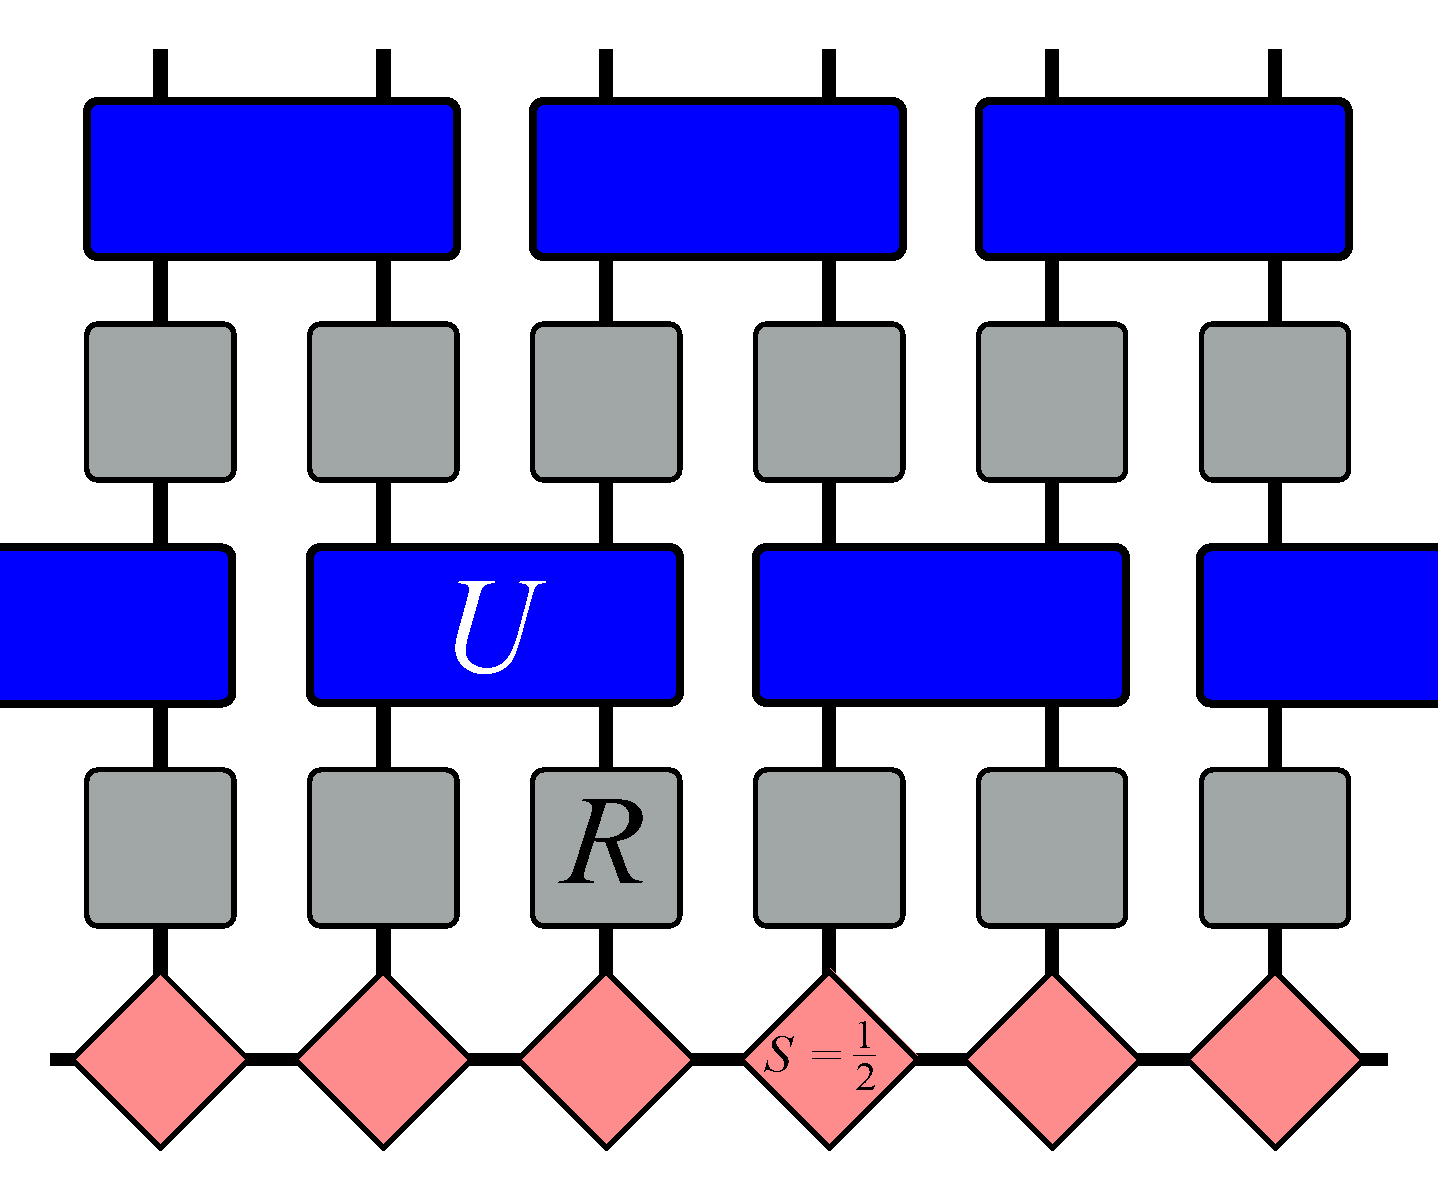
\includegraphics[width=.4\linewidth]{nahum_gates}
	\caption{Quantum circuit, from \cite{Nahum2017}}
\end{figure}
\end{frame}

\begin{frame}{Entanglement Entropy}
\begin{itemize}
	\item Start with $\rho_{AB}= \ket{\Psi}\bra{\Psi}$, $\rho_A = \Tr_B\rho_{AB},$ $\rho_B = \Tr_A\rho_{AB}$
	\item Decompose $\rho_{AB}$ into $\rho_A$, $\rho_B$
	\item Entanglement Entropy: $S(i) = \Tr_A\{\rho_A\log\rho_A\} =
		\Tr_B\{\rho_B\log\rho_B\}$
\end{itemize}
\end{frame}

\begin{frame}{Entanglement Bounds}
\begin{itemize}
	\item For spin $q$, $|S(i) - S(i+1)| \le S(1) \le \log q$
	\item Take log base $q$, $\quad\imp |S(i) - S(i+1)| \le 1$
	\item For $q\to\infty$, arbitrary gates will saturate bound \cite{Nahum2017}
\end{itemize}
\end{frame}

\begin{frame}{Staircase Model}

\begin{figure}
	\centering
	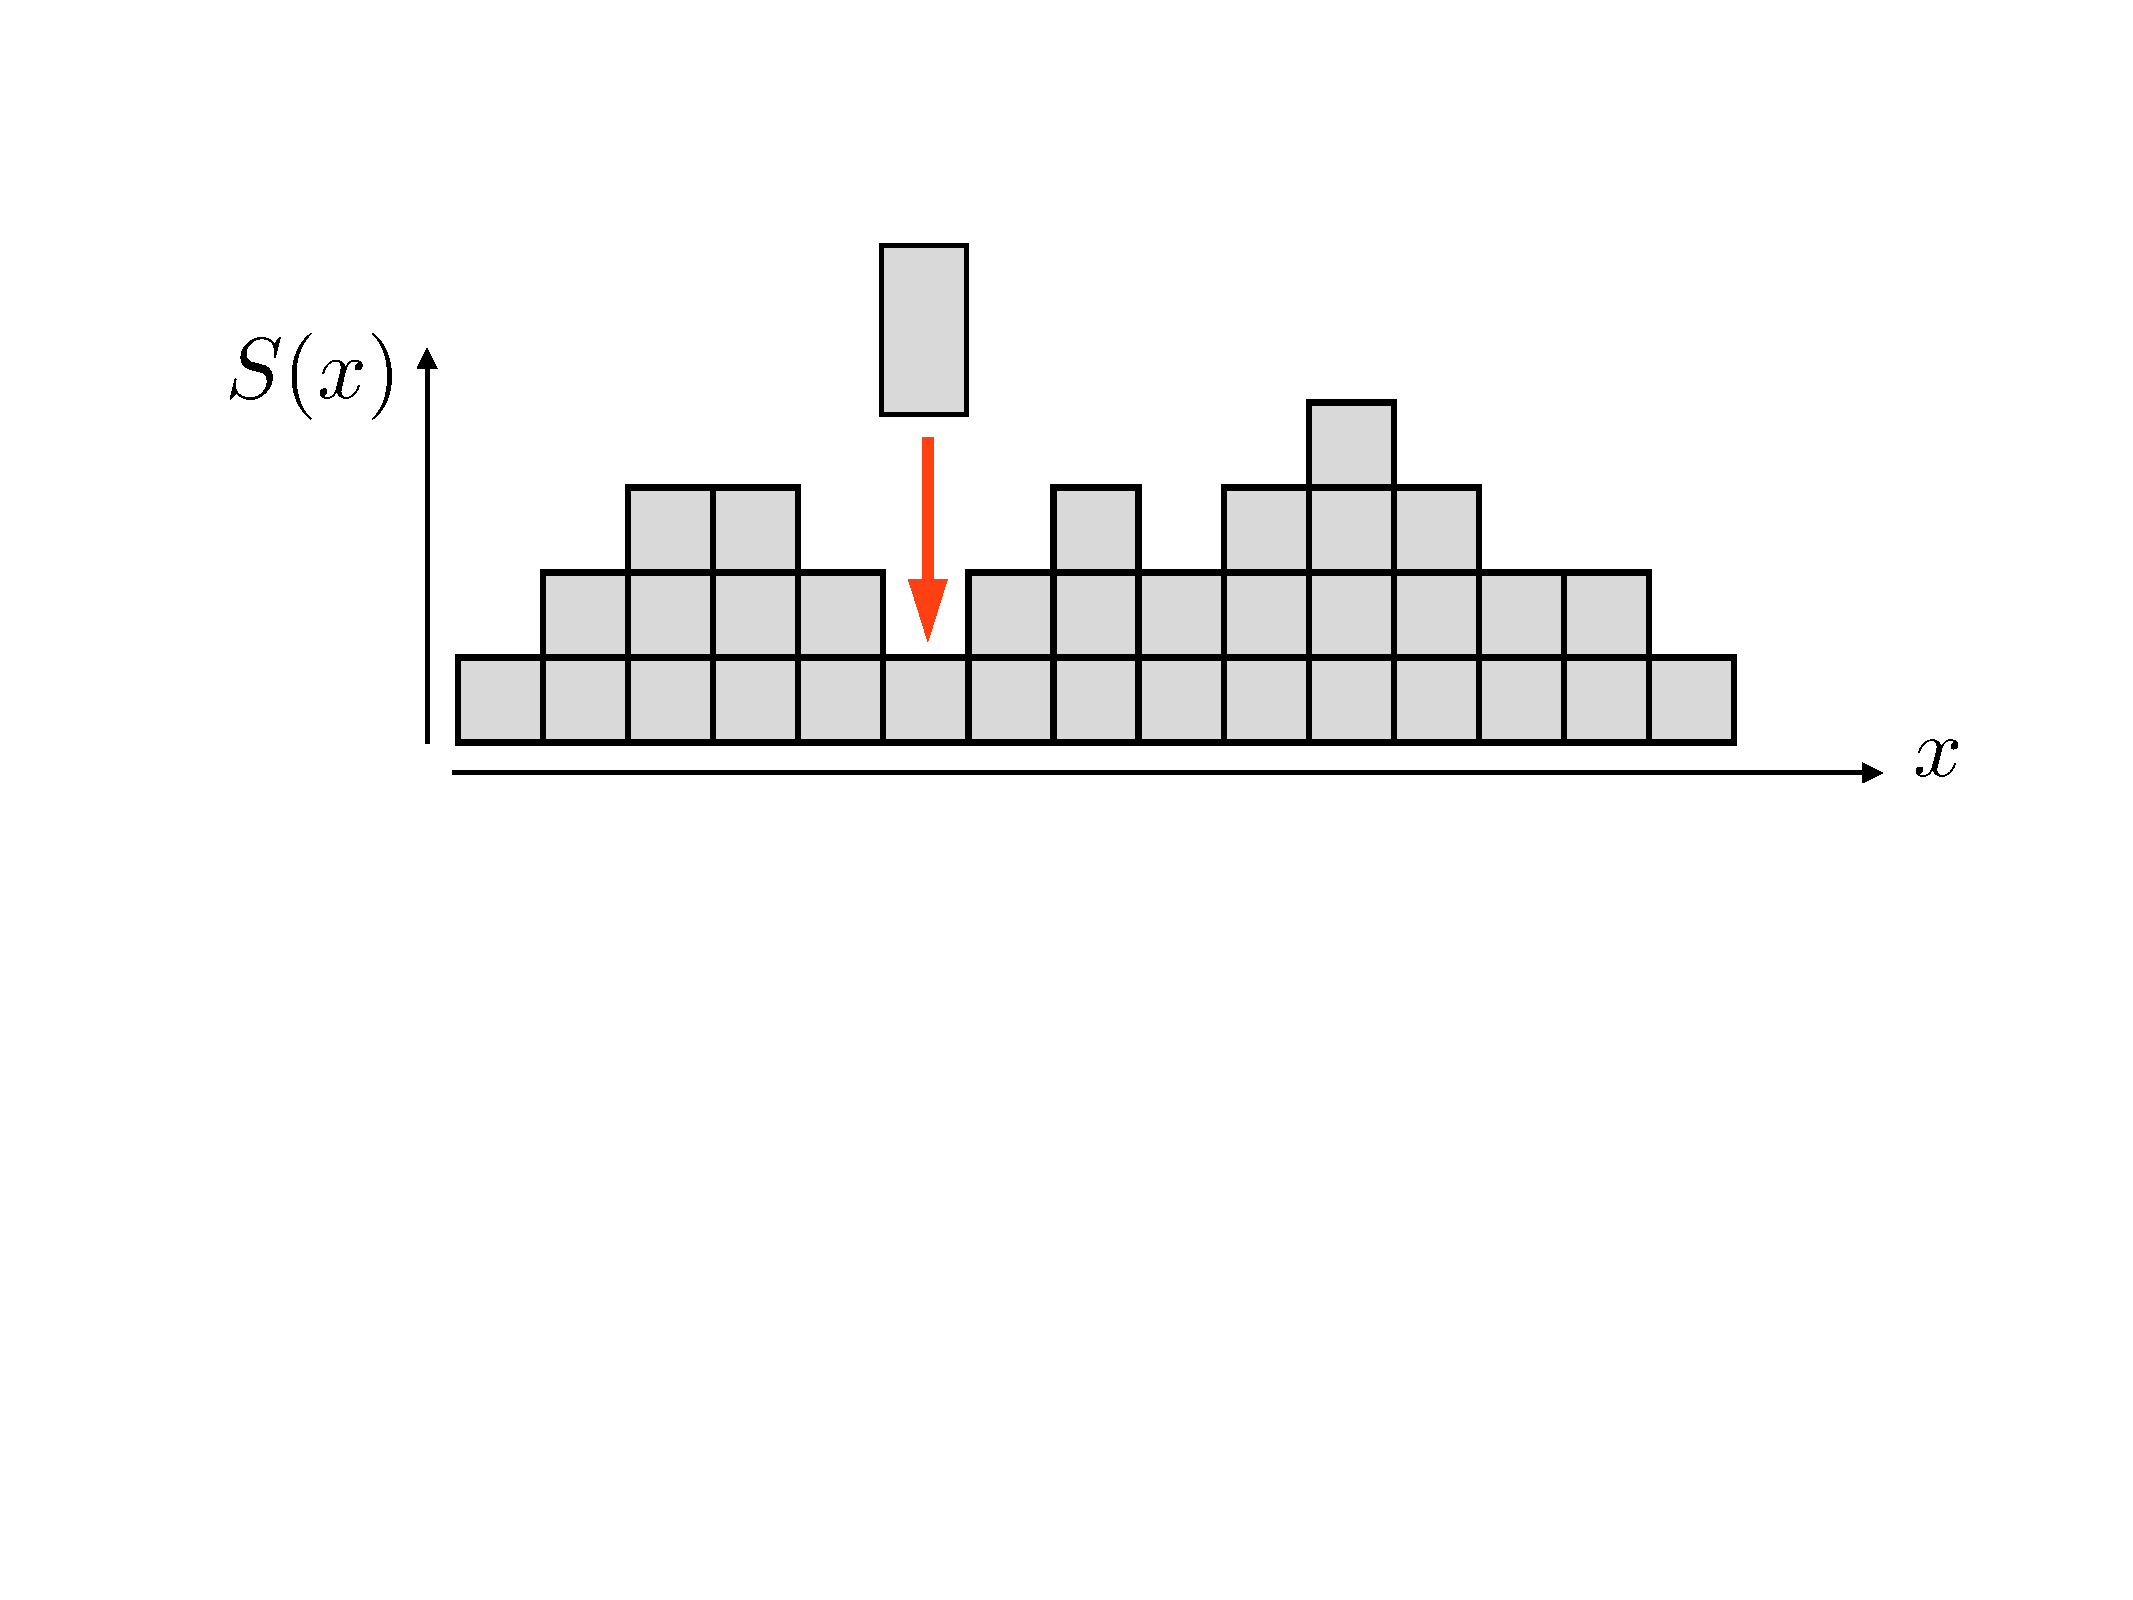
\includegraphics[width=.5\textwidth]{tetris.pdf}
	\caption{\textbf{Tetris-like model for large-$q$ chain.} The gate at cut $x$ adds enough entropy so that $S(x)$ is one greater than either of its neighbors. Taken from~\cite{Nahum2017}.}
	\label{fig:tetris}
\end{figure}

\end{frame}

\begin{frame}{Growth Rates}

After course graining, $\pd{S}{t}$ is a function of $m = \pd{S}{x}$ to first order or for linear entropy.
\begin{figure}
	\centering
	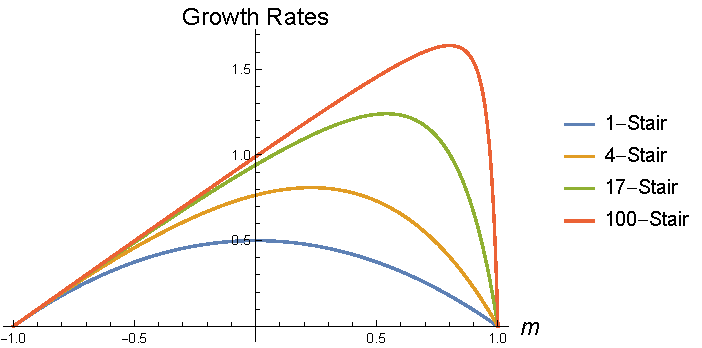
\includegraphics[width=.5\textwidth]{analrates.png}
	\caption{Growth rates for 1-, 4-, 17-, and 100-stairs as a function of slope $m$. As stair length increases, the growth rate asymptotes to the function $\pd{S}{t} = m+1$.}
	\label{fig:growthrates}
\end{figure}
The butterfly velocities are the extremal slopes of this curve \cite{Jonay}.
\end{frame}

\section{Time-Independent Hamiltonian}

\begin{frame}{Time-Independent Hamiltonian}
\begin{itemize}
	\item Back to spin-$\half$
	\item Not relativistic: no limit to information speed
	\item \emph{Most} information still travels at finite speed
	\item Use $H_3 = \vec{\sigma}_1\cdot(\vec{\sigma}_2\times\vec{\sigma}_3)$, the three-site swap
\end{itemize}
\end{frame}

\begin{frame}{Out-of-Time-Order Commutator}
Instead use OTOC:
\begin{align*}
C(i,t) &= \half\ex{|[O_0(t), W_i]|^2}\\
O_0 &= Z\otimes I\otimes I\otimes\cdots\\
O_0(t) &= \e^{-Ht}O_0\e^{-iHt}\\
W_i &= I\otimes I\otimes\cdots W\otimes \cdots I,
\end{align*}
with $W=X,Y,Z$ at site $i$.
\end{frame}

\begin{frame}{Velocity-Dependent Lyapunov Exponent}
For a set velocity, $C(i = vt, t) \sim \e^{\lambda(v)t}$
\begin{figure}
	\centering
	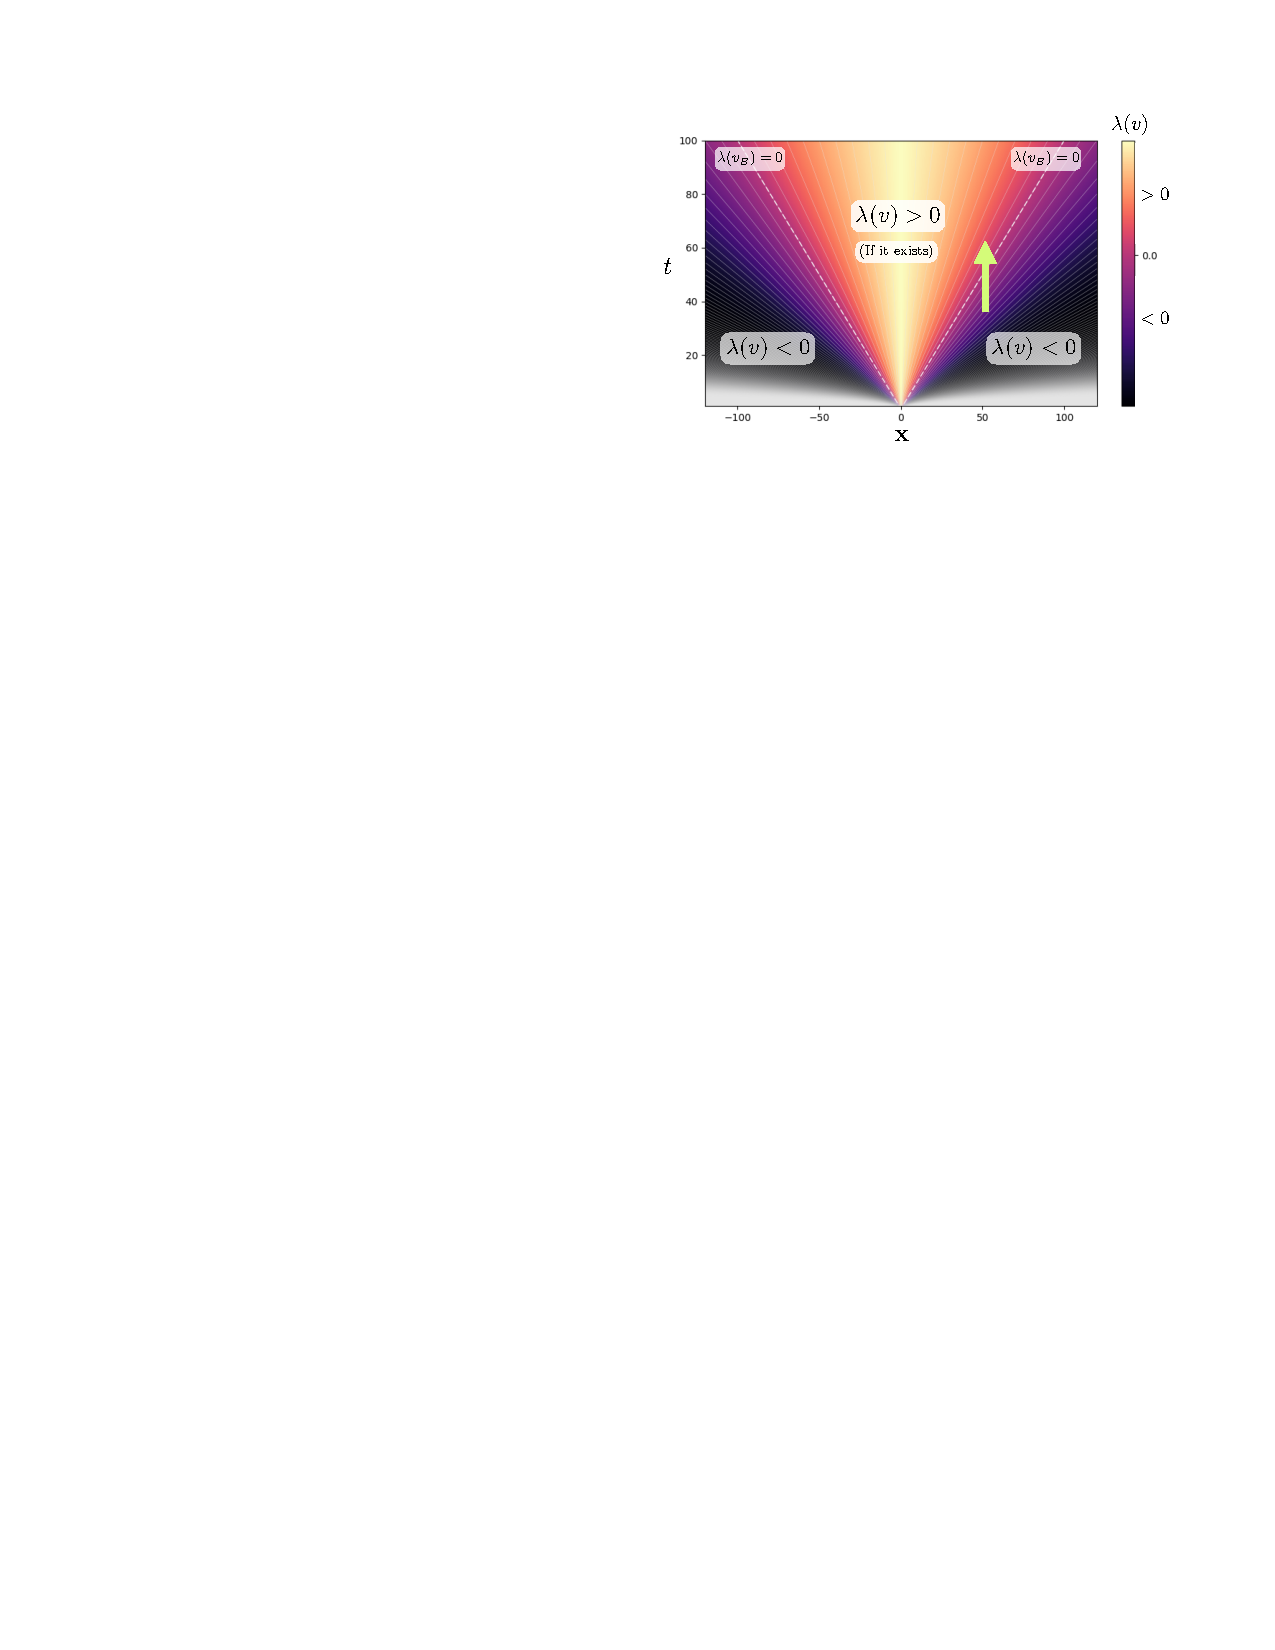
\includegraphics[width=.7\textwidth]{khemani_lambda}
	\caption{Lyapunov exponent at various velocities, from \cite{Khemani2018}}
\end{figure}
\end{frame}

\begin{frame}{Weight at site}

Average of OTOC over $W = X, Y, Z$
\begin{figure}
	\centering
	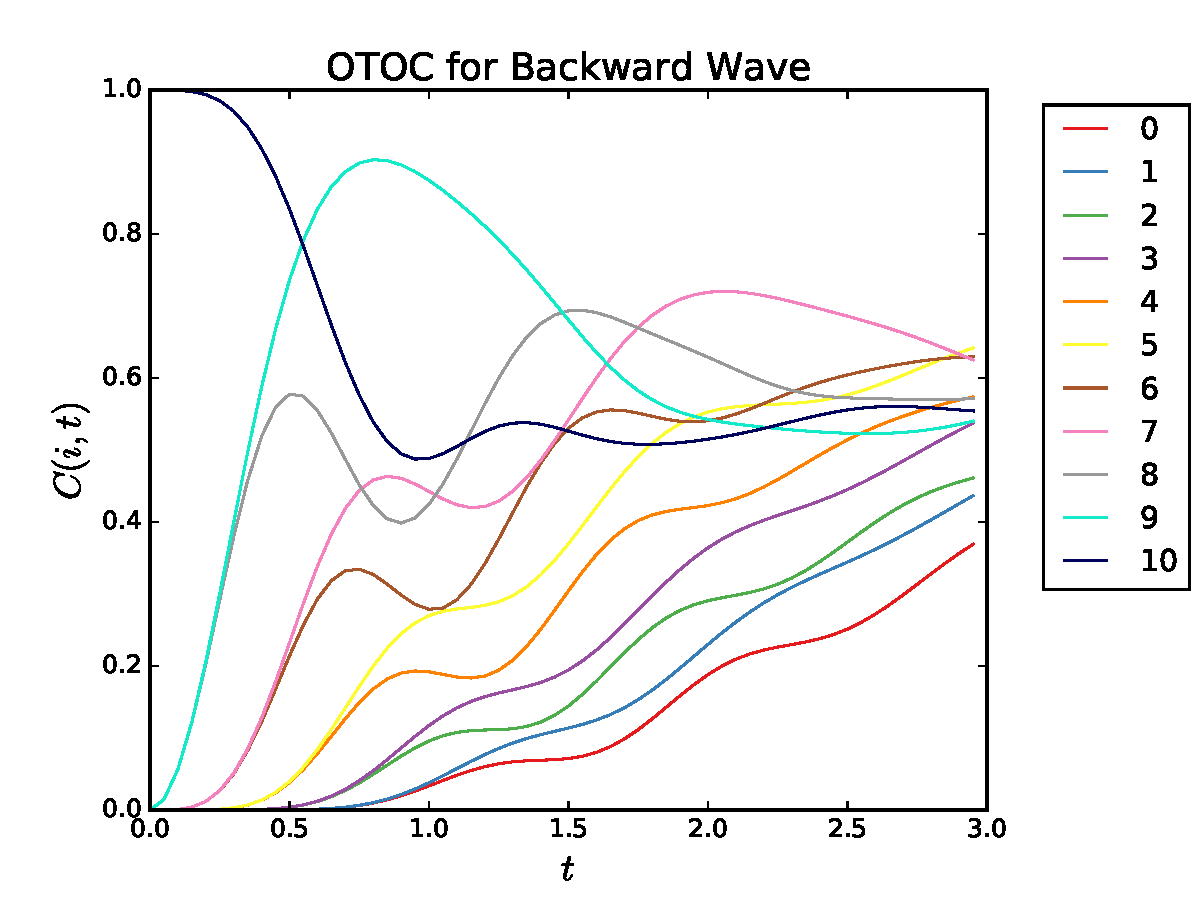
\includegraphics[width=.7\textwidth]{L11end3n20_hereback}
	\caption{Weight of operators that begin on site $i$.}
	\label{fig:L11end3n20back}
\end{figure}

\end{frame}

\begin{frame}{OTOC}

Looking for asymmetry
\begin{figure}
	\centering
	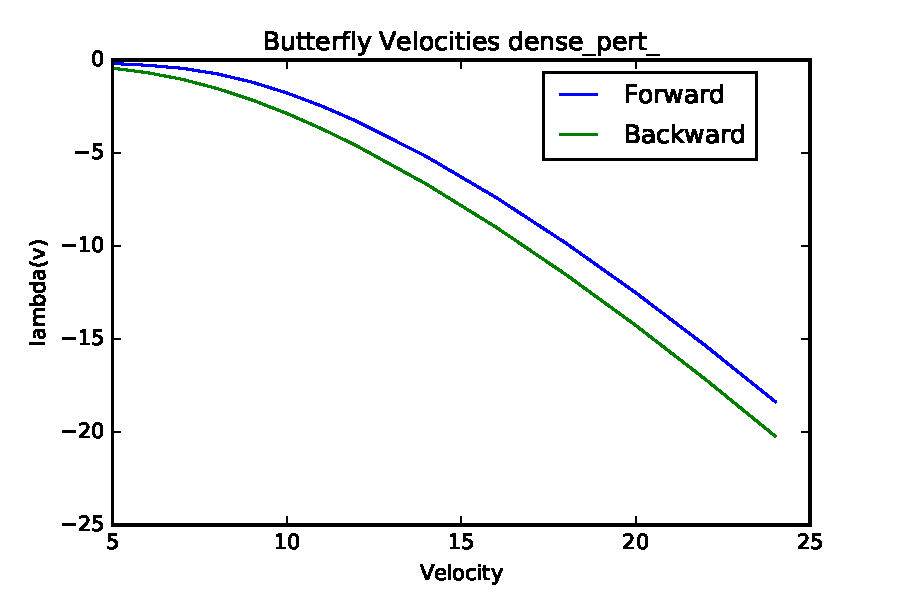
\includegraphics[width=.7\textwidth]{balanced_butterfly_dense_pert_L11}
	\caption{Calculating Butterfly Velocity from early time evolution.}
\end{figure}

\end{frame}

\begin{frame}
\nocite{}
\frametitle{References}
\footnotesize{
	\bibliographystyle{abbrv}
	\bibliography{../LaTeX/bib.bib}
}
\end{frame}

\end{document} 